\section{Functional Modeling}

FUNCTIONAL MODELING SHIFTS OUR FOCUS FROM THE USER'S ACTIONS TO HOW THE SYSTEM STORES, STRUCTURES, AND MOVES DATA. WHILE OUR USE CASES SHOW WHAT ACTORS DO, FUNCTIONAL MODELS SHOW HOW OUR BACKEND COORDINATES EVERYTHING. FOR SMARTEXAM, WE MUST MANAGE CONSTANT WEBSOCKET TELEMETRY, COMPRESSED WEBCAM SCREENSHOTS, AND DOCKER COMPILATIONS WITHOUT SLOWING DOWN THE SERVER. WE ALSO NEED TO GUARANTEE THAT DATABASE RECORDS, SUCH AS GRADES AND AUDIT TRAILS, REMAIN CONSISTENT AND SECURE.

HERE, WE LAY OUT OUR RELATIONAL DATABASE SCHEMA AND OUR DATA FLOW PIPELINES. WE PRESENT OUR ENTITY RELATIONSHIP DIAGRAM (ERD) IMPLEMENTED ON NEON POSTGRESQL. WE ALSO USE DATA FLOW DIAGRAMS (DFDS) AT THREE LEVELS OF DETAIL TO MAP HOW TELEMETRY AND GRADES TRAVEL THROUGH THE SYSTEM.

\subsection{Entity Relationship Diagram}

WE CHOSE A RELATIONAL DATABASE MODEL (NEON POSTGRESQL) OVER NOSQL FOR SMARTEXAM. WE NEED STRICT SCHEMAS AND REFERENTIAL CONSTRAINTS TO MAKE SURE STUDENT GRADES AND LOGS ARE NEVER LOST OR CORRUPTED \cite{er_diagram_lucidchart}. NEON POSTGRESQL'S SERVERLESS AUTO-SCALING HELPS US HANDLE THE MASSIVE CONNECTION SPIKES WHEN A WHOLE CLASS STARTS AN EXAM.

TO AVOID ANOMALIES, WE NORMALIZED THE DATABASE TO THIRD NORMAL FORM (3NF). STUDENT ACCOUNTS, SEATING LAYOUTS, AND GRADING METRICS SIT IN SEPARATE TABLES. FOREIGN KEY RELATIONSHIPS LINK THEM TOGETHER, PREVENTING DUPLICATED RECORDS. WE USE INDEXES ON FREQUENTLY SEARCHED COLUMNS TO SPEED UP DASHBOARD QUERIES DURING EXAMS.

FIGURE~\ref{fig:erd_diagram} SHOWS OUR ERD LAYOUT. IT FEATURES 14 TABLES THAT TRACK THE SYSTEM'S COMPLETE STATE.

\begin{figure}[H]
\centering
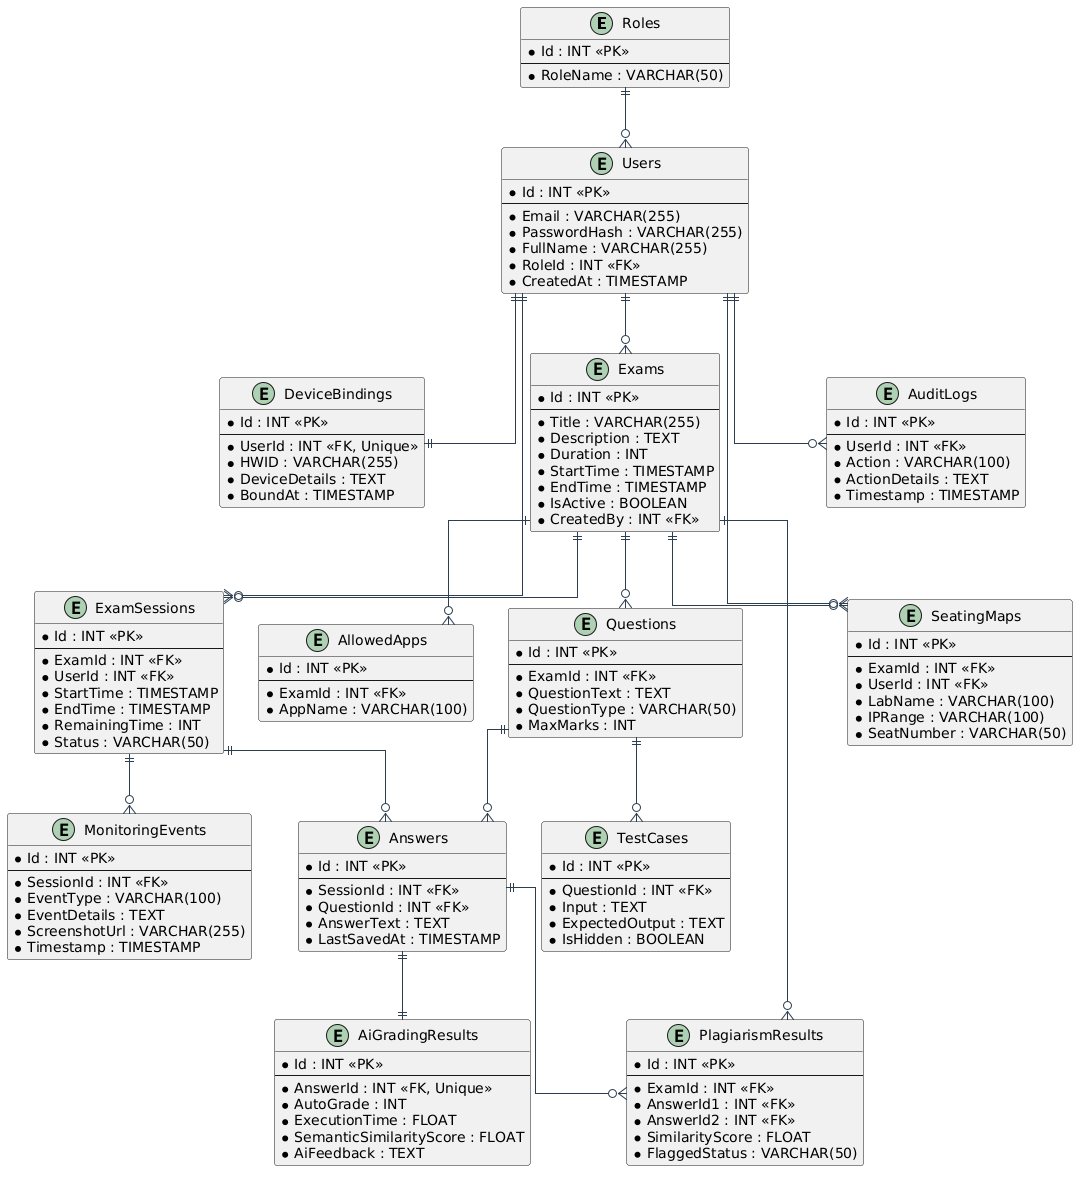
\includegraphics[width=0.97\linewidth]{Figures/erd_diagram.png}
\caption{Entity Relationship Diagram (ERD) of the SmartExam Database Schema}
\label{fig:erd_diagram}
\end{figure}

OUR DATABASE SCHEMA IS STRUCTURED AROUND THESE KEY TABLES:
\begin{enumerate}
    \item \textbf{Roles Table (\texttt{Roles}):} STORES ACCESS LEVELS (STUDENT, TEACHER, ADMIN). IT CONTAINS A PRIMARY KEY \texttt{Id} AND \texttt{RoleName}.
    \item \textbf{Users Table (\texttt{Users}):} MANAGES STUDENT, TEACHER, AND ADMINISTRATOR PROFILES. IT STORES NAMES, HASHED PASSWORDS, AND LINKS BACK TO THE \texttt{Roles} TABLE.
    \item \textbf{Device Bindings Table (\texttt{DeviceBindings}):} PAIRS A STUDENT'S \texttt{UserId} WITH THEIR UNIQUE WORKSTATION \texttt{HWID} HASH. THIS ONE-TO-ONE MAPPING BLOCKS STUDENTS FROM LOGGING IN FROM UNAUTHORIZED MACHINES.
    \item \textbf{Exams Table (\texttt{Exams}):} STORES EXAM METADATA LIKE TITLES, DURATIONS, START/END WINDOWS, AND ALLOWED APPLICATION LISTS.
    \item \textbf{Questions Table (\texttt{Questions}):} STORES CODING AND THEORY QUESTIONS FOR EACH EXAM.
    \item \textbf{Test Cases Table (\texttt{TestCases}):} HOLDS THE INPUT AND EXPECTED OUTPUT PAIRS USED BY THE COMPILATION ENGINE TO EVALUATE STUDENT CODE.
    \item \textbf{Allowed Applications Table (\texttt{AllowedApps}):} WHITELISTS PERMITTED DESKTOP EXECUTABLES (E.G., \texttt{code.exe}).
    \item \textbf{Seating Maps Table (\texttt{SeatingMaps}):} BINDS REGISTERED CANDIDATES TO SPECIFIC LABORATORY SEATING ARRANGEMENTS AND IP ADDRESSES.
    \item \textbf{Exam Sessions Table (\texttt{ExamSessions}):} TRACKS THE STATE OF ACTIVE EXAMS, RECORDING REMAINING DURATIONS AND SESSION STATUSES.
    \item \textbf{Answers Table (\texttt{Answers}):} STORES STUDENT RESPONSES. THE CLIENT AUTO-SAVES CODE DRAFTS HERE EVERY 10 SECONDS.
    \item \textbf{Monitoring Events Table (\texttt{MonitoringEvents}):} STORES FLAGGED VIOLATIONS, PROCESS LOGS, AND SCREENSHOTS CAPTURED DURING LOCKDOWN.
    \item \textbf{AI Grading Results Table (\texttt{AiGradingResults}):} HOLDS AUTOMATED SCORES, COMPILE TIMES, AND SIMILARITY EVALUATIONS.
    \item \textbf{Plagiarism Results Table (\texttt{PlagiarismResults}):} STORES SIMILARITY SCORES GENERATED BY OUR PAIRWISE PLAGIARISM CHECKER.
    \item \textbf{Audit Logs Table (\texttt{AuditLogs}):} AN IMMUTABLE, READ-ONLY LOG OF TEACHER OVERRIDES AND ADMIN CONFIGURATIONS.
\end{enumerate}

\subsubsection{Key Entity Relationships}
We defined three primary relationship structures in our database:
\begin{itemize}
    \item \textbf{One-to-One:} A student user maps to exactly one device binding. This locks their credentials to a single workstation.
    \item \textbf{One-to-Many:} An exam contains multiple questions, whitelisted apps, seating limits, and student sessions.
    \item \textbf{Junction-Based Mappings:} Tables like seating allocations and grades act as junctions, linking users, questions, and sessions to keep records searchable.
\end{itemize}

\subsection{Data Flow Diagram}

4 Data Flow Diagrams The SmartExam system's data flow represents the movement of information as it enters, moves through, and leaves SmartExam. We adopt the Gane-Sarson notation for DFD diagrams where: Processes are represented by rounded rectangles, External entities are represented by squares, Data flows are represented by arrows, and Data stores are represented by open rectangles. The data flow of SmartExam has been mapped at three levels: context diagram (Level 0), subsystem overview (Level 1), and detailed processing (Level 2).

\subsubsection{DFD Level 0}

Figure~\ref{fig:dfd_level_0} illustrates the DFD Level 0 or Context Diagram, which defines the system boundaries for SmartExam and represents the entire platform as a single process in direct communication with its four primary external entities.

\begin{figure}[H]
\centering
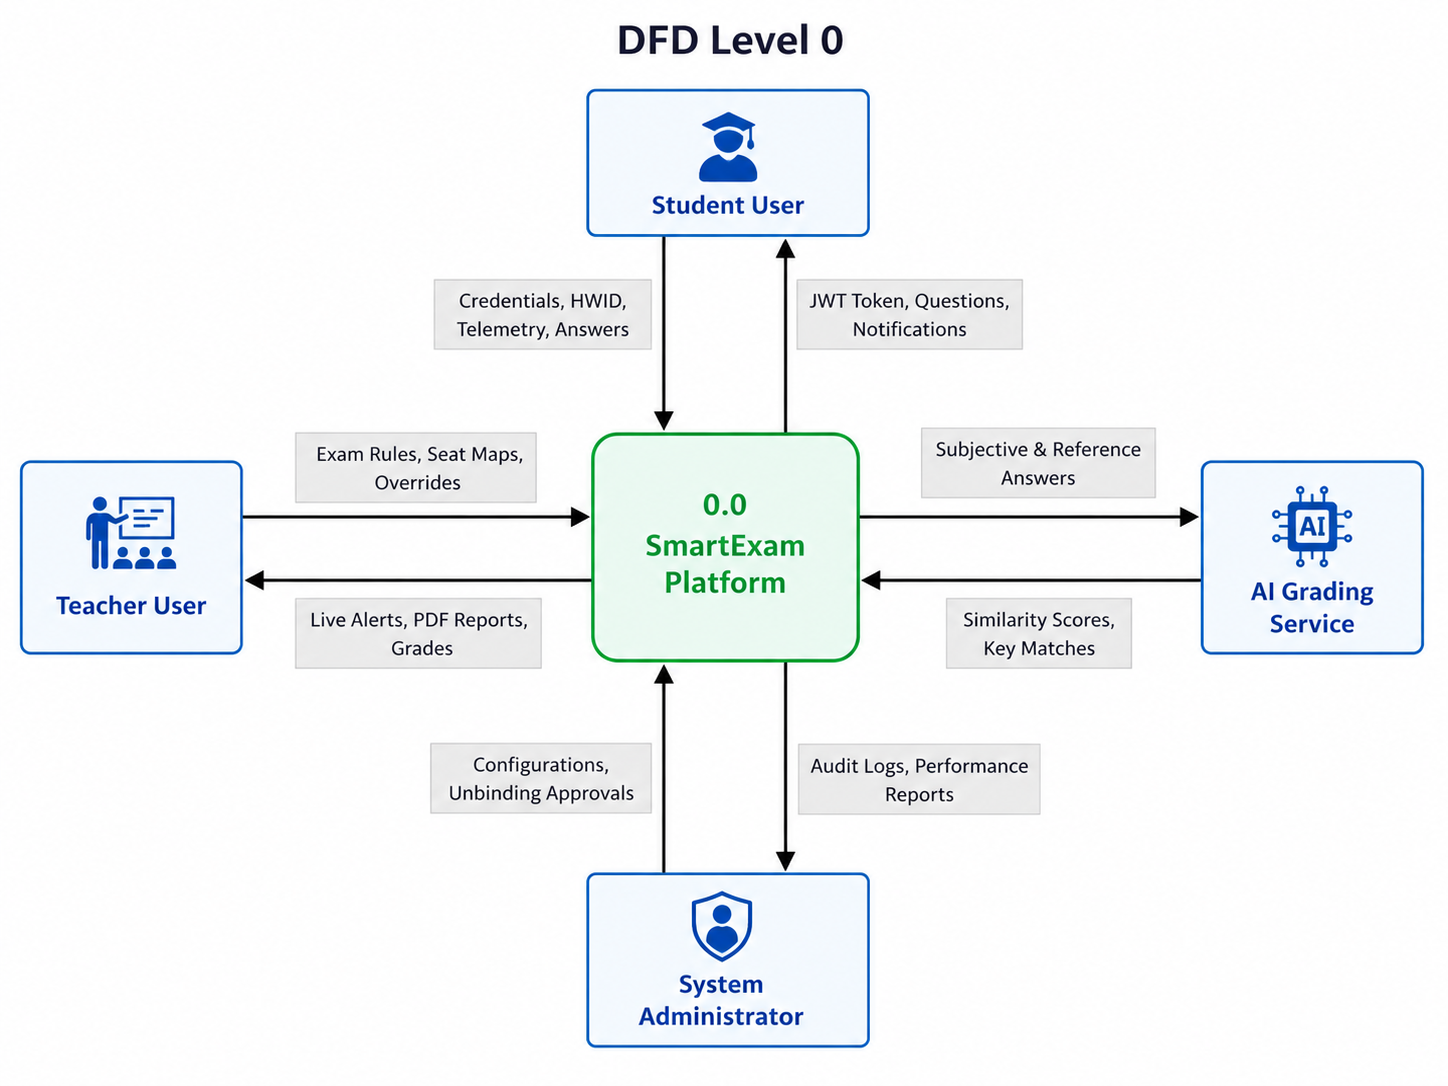
\includegraphics[width=0.97\linewidth]{Figures/dfd_level_0.png}
\caption{Data Flow Diagram (DFD) Level 0 --- Context Diagram}
\label{fig:dfd_level_0}
\end{figure}

The boundary flows indicated in Figure~\ref{fig:dfd_level_0} are:
\begin{itemize}
    \item \textbf{Student User:} Student provides username, password, HWID hash, diagnostic status, process logs, and submission answers. Student receives JWT token, diagnostic clearance, questions, and receipt of answers.
    \item \textbf{Teacher User:} Teacher configures allowed applications, seating arrangements, scheduling and sends commands to control exams. Teacher receives student monitoring reports, warnings, and grading summary sheets.
    \item \textbf{System Administrator:} Administrator provides settings, role configurations and control of hardware bindings. System Administrator receives system logs, status of devices and network devices.
    \item \textbf{AI Grading Service:} AI service receives student and reference text answers. AI service provides text similarities and grading data.
\end{itemize}

\subsubsection{DFD Level 1}

The DFD Level 1 disaggregates the central process in Figure~\ref{fig:dfd_level_0} into 5 main functional components, namely:

\begin{figure}[H]
\centering
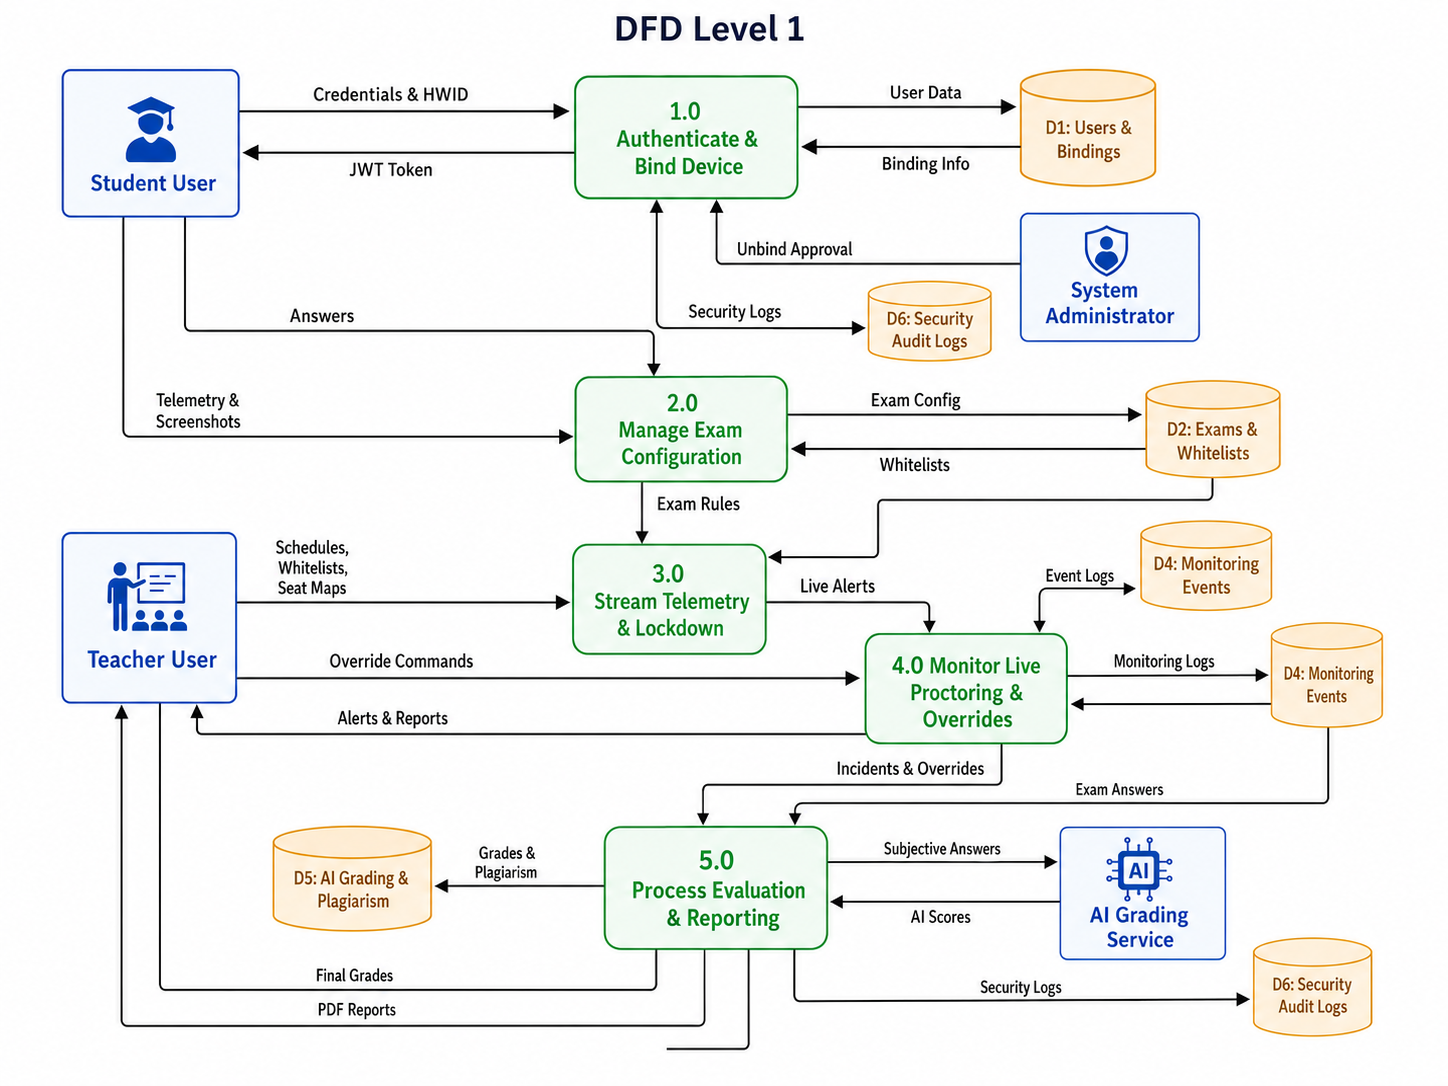
\includegraphics[width=0.97\linewidth]{Figures/dfd_level_1.png}
\caption{Data Flow Diagram (DFD) Level 1 --- Subsystem Overview}
\label{fig:dfd_level_1}
\end{figure}

\begin{enumerate}
    \item \textbf{Authentication and Device Binding (Process 1.0):} Authenticates the HWID and device signature. On successful verification, a unique JSON Web Token (JWT) is generated and sent to the client.
    \item \textbf{Exam Setup and Access Control (Process 2.0):} Sets exam parameters like time, question difficulty and list of allowed applications. Exam configurations, whitelists and seats information is fed into matching student clients.
    \item \textbf{Lockdown and Telemetry Streaming (Process 3.0):} Monitors client systems and captures running processes, and system status. Any suspicious activities such as face switching or unauthorized application usage is logged. All monitored data is streamed to a central storage which is also available for a viewing tool for instructors.
    \item \textbf{Live Proctoring and Overrides (Process 4.0):} The system uses WebSockets to stream and display captured telemetry in real-time at the instructor's terminal. It also allows authorized personnel to manually control an ongoing examination or unlock the system based on justified requests.
    \item \textbf{Evaluation, Plagiarism, and Reporting (Process 5.0):} Collects the final answers from all participating students. Each of the answer submissions are then sent for automated grading by the AI service and subjected to a plagiarism check using a pairwise comparison approach with existing submissions and online materials (e.g. through text comparisons with student and instructor databases, and with text from common online resources). Final marks for each assessment, and a plagiarism report are generated.
\end{enumerate}

\subsubsection{DFD Level 2}

We zoom in on telemetry streaming and exam evaluation to show the exact process steps inside Process 3.0 and Process 5.0 (Figure~\ref{fig:dfd_level_2}).

\begin{figure}[H]
\centering
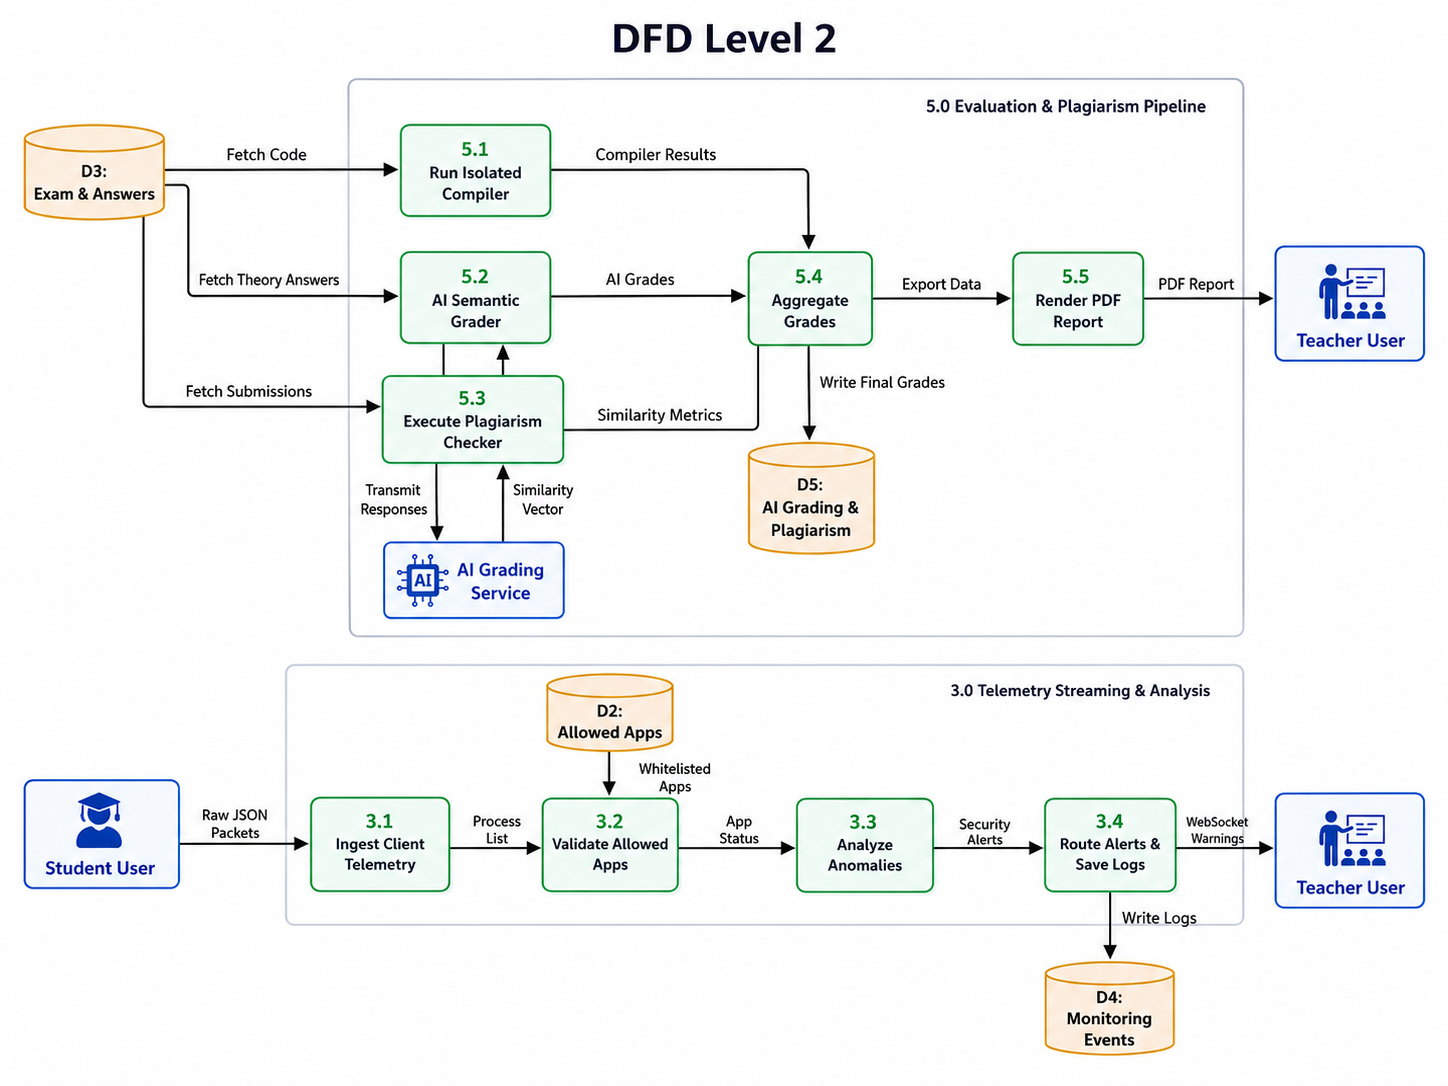
\includegraphics[width=0.97\linewidth]{Figures/dfd_level_2.png}
\caption{Data Flow Diagram (DFD) Level 2 --- Telemetry and Evaluation Processing}
\label{fig:dfd_level_2}
\end{figure}

The details in Figure~\ref{fig:dfd_level_2} trace:
\begin{enumerate}
    \item \textbf{Telemetry Streaming and Analysis (Process 3.1 to 3.4):} Process 3.1 ingests client JSON packets over WebSocket. Process 3.2 matches running apps against whitelisted settings. Process 3.3 runs anomaly tests (e.g. face presence, tab switching). Process 3.4 writes events to \texttt{MonitoringEvents} and pushes live alerts to the teacher's stream.
    \item \textbf{Evaluation and Plagiarism Checking (Process 5.1 to 5.5):} Process 5.1 runs submitted files inside sandboxed Docker containers to test code against inputs. Process 5.2 calculates similarity vectors for theory text. Process 5.3 performs pairwise comparisons across the class database to catch copy-paste plagiarism. Process 5.4 aggregates these scores into the database, and Process 5.5 compiles the QuestPDF template.
\end{enumerate}

These Level 2 pipelines form the engine of SmartExam. By documenting data transforms at this level, we ensure the backend can process active streams without lag during exam sessions.